% A1 poster — Projektarbete SF1693, KTH VT 2026
% OU-processen, Fokker–Planck-ekvationen och Vasicek-modellen
% Radial pentagon layout with central hub.
%
% Build with:  pdflatex poster.tex   (or xelatex / lualatex)

\documentclass[20pt]{extarticle}

\usepackage[paperwidth=594mm,paperheight=841mm,margin=20mm]{geometry}

\usepackage[utf8]{inputenc}
\usepackage[T1]{fontenc}
\usepackage[swedish]{babel}
\usepackage{lmodern}

\usepackage{graphicx}
\usepackage{amsmath, amssymb}
\usepackage{xcolor}
\usepackage{tikz}
\usetikzlibrary{calc}

% --- Stora poster-typsnittsstorlekar ----------------------------------
\newcommand{\veryHuge}{\fontsize{72}{86}\selectfont}
\newcommand{\posterHuge}{\fontsize{56}{68}\selectfont}

% --- KTH-inspirerad färgpalett ----------------------------------------
\definecolor{KTHblue}{RGB}{25,84,166}
\definecolor{KTHaccent}{RGB}{98,146,190}

\renewcommand{\familydefault}{\sfdefault}
\pagestyle{empty}
\setlength{\parindent}{0pt}
\setlength{\parskip}{0.4em}

\begin{document}

% ============== TOPPBANNER: logga vänster, titel mitt =================
\noindent
\begin{minipage}[c]{90mm}
  
\includegraphics[width=85mm]{kth.png}
\end{minipage}%
\hfill
\begin{minipage}[c]{\dimexpr\linewidth-95mm\relax}
  \begin{center}
    {\color{KTHblue}\posterHuge\textbf{Ornstein--Uhlenbeck-processen}}\\[0.4em]
    {\color{KTHblue}\Huge\textbf{Fokker--Planck-ekvationen och Vasicek-modellen}}\\[1em]
    {\Large Carl Gustaf Bril \quad Viggo Forsman \quad Hjalmar Lindström \quad Gabriel Svärdson Wächter}\\[0.3em]
    {\large Projektarbete SF1693 -- KTH, Vårterminen 2026}
  \end{center}
\end{minipage}

\vspace{0.5em}
{\color{KTHblue}\rule{\linewidth}{4pt}}
\vspace{1em}

% ============== RADIAL PENTAGON LAYOUT ================================
\begin{center}
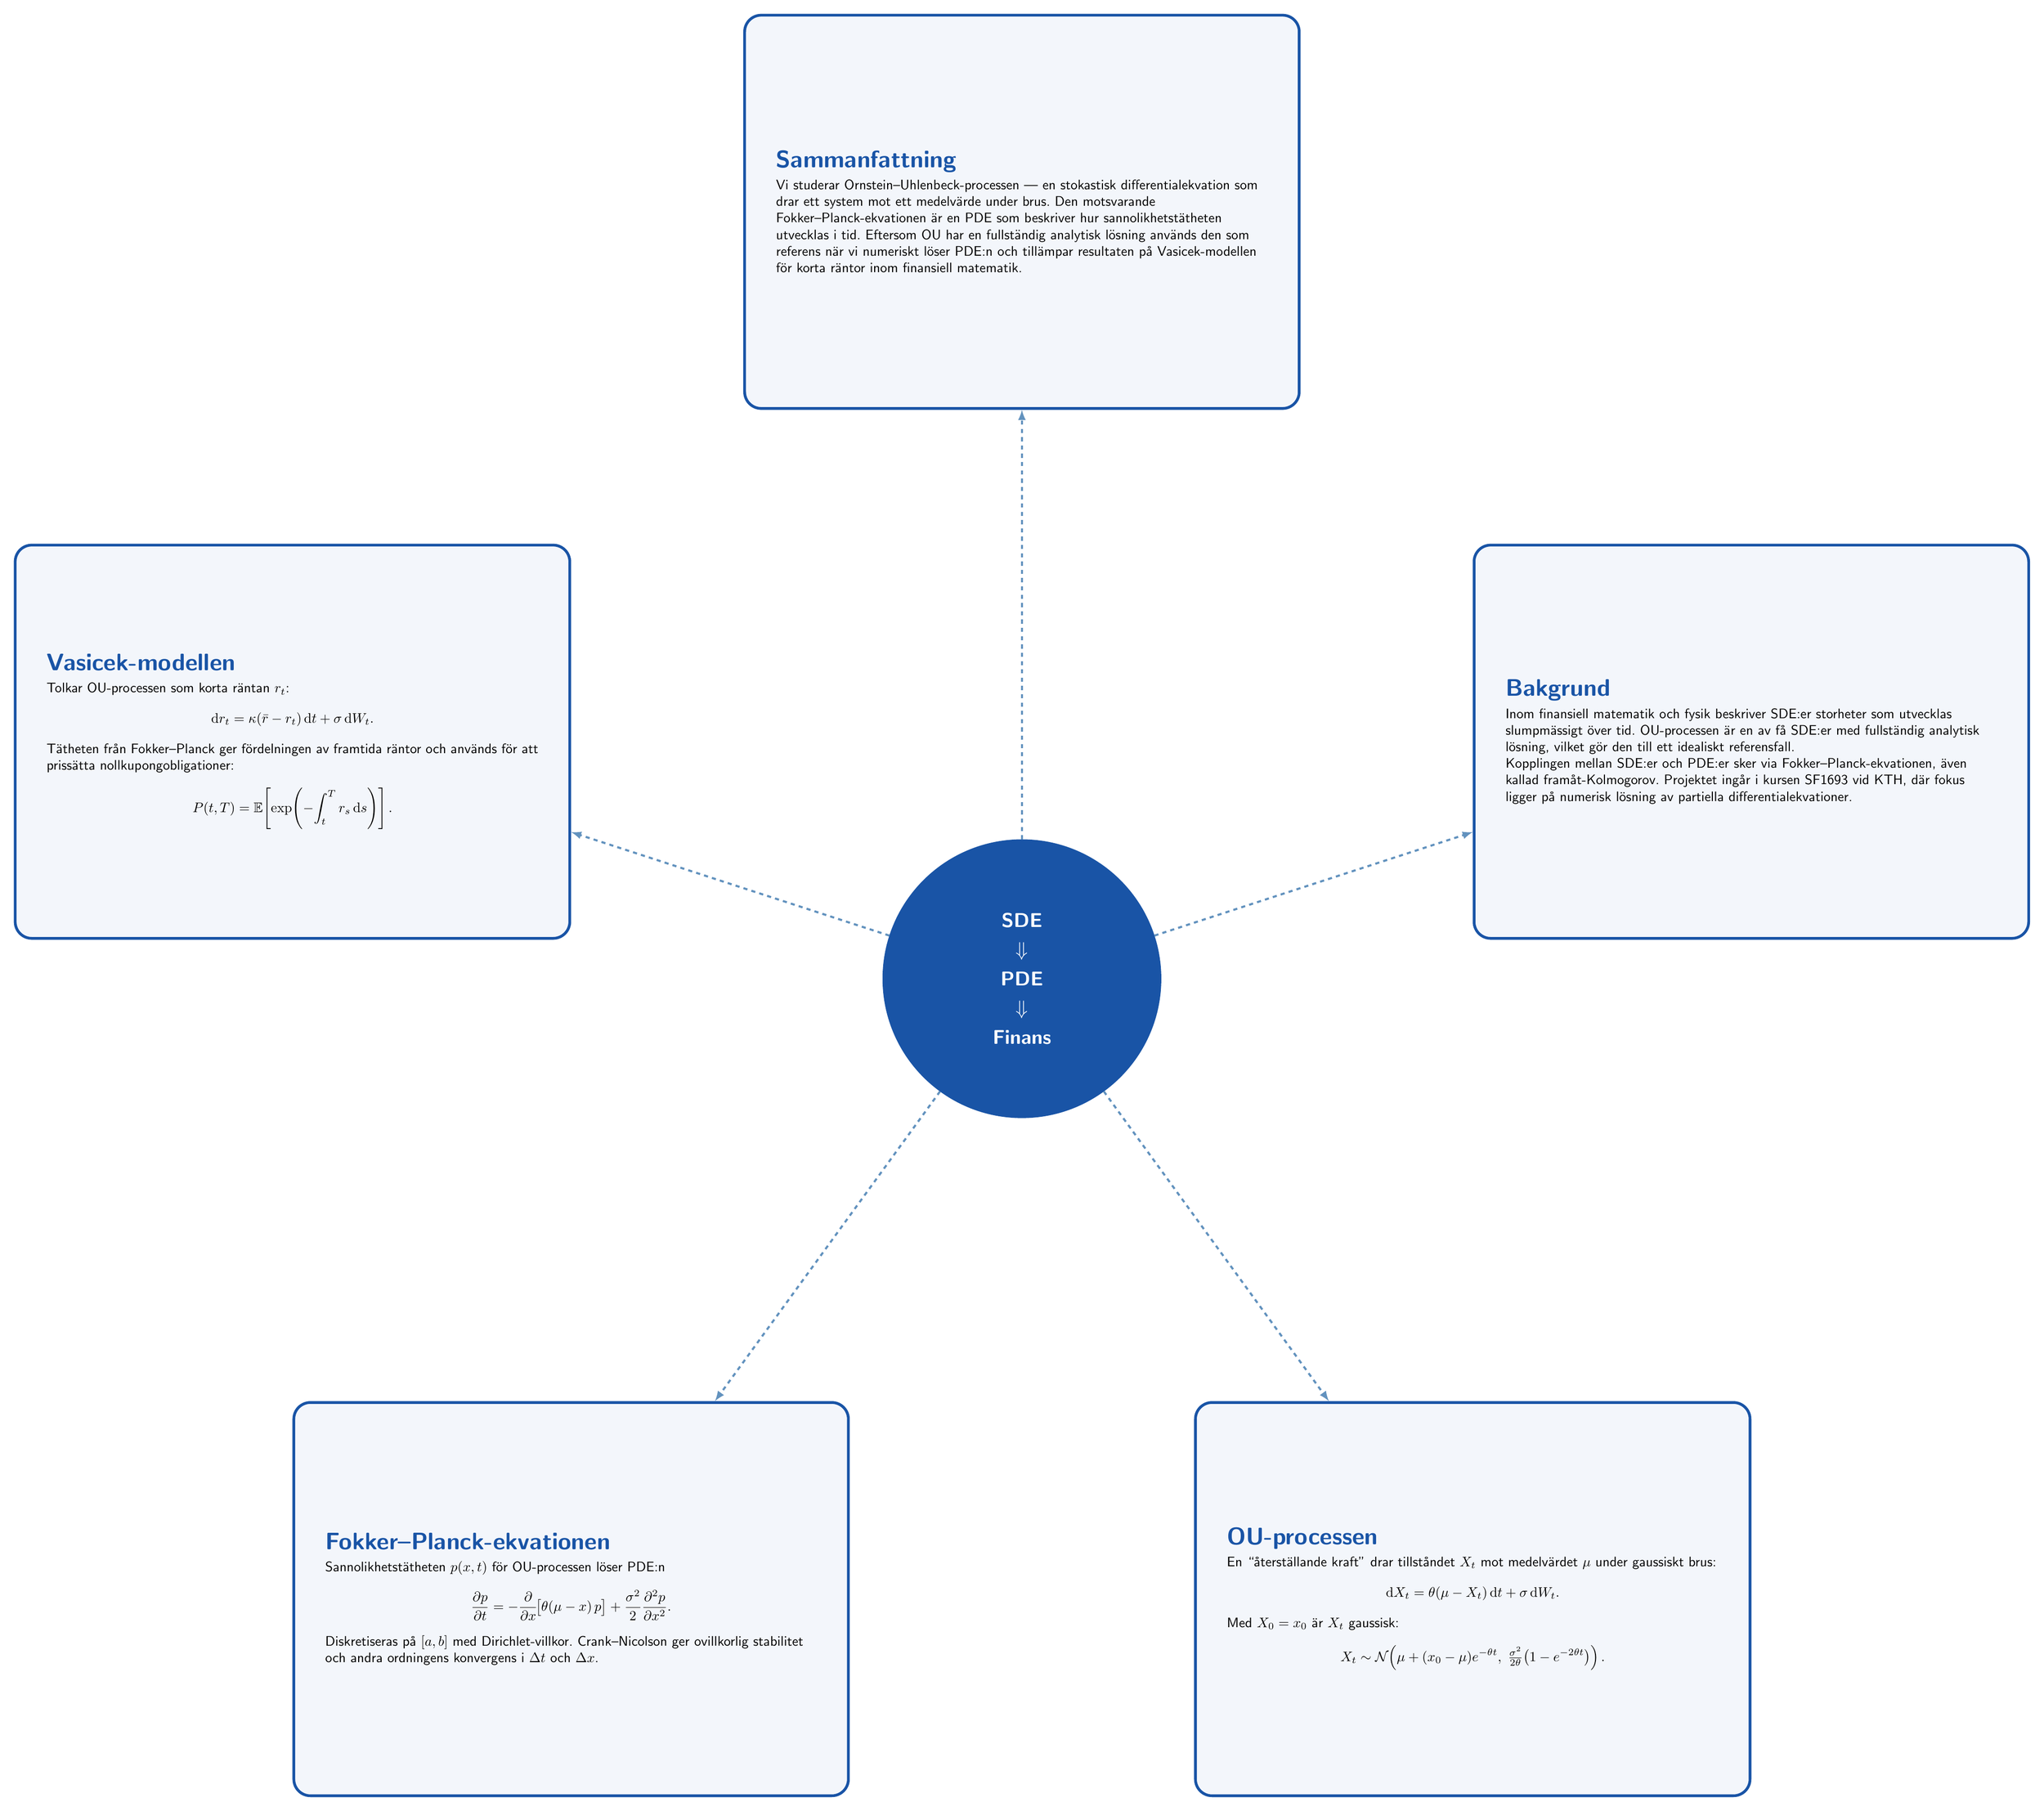
\begin{tikzpicture}[
  sectionnode/.style={
    rectangle, rounded corners=12pt,
    draw=KTHblue, line width=2pt,
    fill=KTHblue!5,
    text width=12.5cm,
    minimum height=10cm,
    align=flush left,
    inner sep=8mm,
    font=\normalsize,
  },
  centerhub/.style={
    circle, draw=KTHblue, line width=2.5pt,
    fill=KTHblue, text=white,
    minimum size=7cm,
    align=center,
    inner sep=2mm,
    font=\Large\bfseries,
  },
  spoke/.style={
    KTHaccent, line width=1.5pt, dashed, -latex,
  },
]

\def\R{19.5cm}

% --- Center hub: project flow ---------------------------------------
\node[centerhub] (hub) at (0,0) {%
  SDE\\[0.2em]
  $\Downarrow$\\[0.2em]
  PDE\\[0.2em]
  $\Downarrow$\\[0.2em]
  Finans
};

% --- 1. Sammanfattning -- top (90 deg) ------------------------------
\node[sectionnode] (s1) at (90:\R) {%
  {\color{KTHblue}\LARGE\bfseries Sammanfattning}\\[0.4em]
  Vi studerar Ornstein--Uhlenbeck-processen --- en stokastisk
  differentialekvation som drar ett system mot ett medelvärde
  under brus. Den motsvarande Fokker--Planck-ekvationen är en PDE
  som beskriver hur sannolikhetstätheten utvecklas i tid. Eftersom
  OU har en fullständig analytisk lösning används den som referens
  när vi numeriskt löser PDE:n och tillämpar resultaten på
  Vasicek-modellen för korta räntor inom finansiell matematik.
};

% --- 2. Bakgrund -- upper right (18 deg) ----------------------------
\node[sectionnode] (s2) at (18:\R) {%
  {\color{KTHblue}\LARGE\bfseries Bakgrund}\\[0.4em]
  Inom finansiell matematik och fysik beskriver SDE:er storheter
  som utvecklas slumpmässigt över tid. OU-processen är en av få
  SDE:er med fullständig analytisk lösning, vilket gör den till
  ett idealiskt referensfall.

  Kopplingen mellan SDE:er och PDE:er sker via
  Fokker--Planck-ekvationen, även kallad framåt-Kolmogorov.
  Projektet ingår i kursen SF1693 vid KTH, där fokus ligger på
  numerisk lösning av partiella differentialekvationer.
};

% --- 3. OU-processen -- lower right (306 deg) -----------------------
\node[sectionnode] (s3) at (306:\R) {%
  {\color{KTHblue}\LARGE\bfseries OU-processen}\\[0.4em]
  En ``återställande kraft'' drar tillståndet $X_t$ mot
  medelvärdet $\mu$ under gaussiskt brus:
  \[
    \mathrm{d}X_t = \theta(\mu - X_t)\,\mathrm{d}t + \sigma\,\mathrm{d}W_t.
  \]
  Med $X_0 = x_0$ är $X_t$ gaussisk:
  \[
    X_t \sim \mathcal{N}\!\left(
      \mu + (x_0-\mu)e^{-\theta t},\;
      \tfrac{\sigma^2}{2\theta}\bigl(1 - e^{-2\theta t}\bigr)
    \right).
  \]
};

% --- 4. Fokker--Planck-ekvationen -- lower left (234 deg) -----------
\node[sectionnode] (s4) at (234:\R) {%
  {\color{KTHblue}\LARGE\bfseries Fokker--Planck-ekvationen}\\[0.4em]
  Sannolikhetstätheten $p(x,t)$ för OU-processen löser PDE:n
  \[
    \frac{\partial p}{\partial t}
      = -\frac{\partial}{\partial x}\!\bigl[\theta(\mu - x)\,p\bigr]
      + \frac{\sigma^2}{2}\frac{\partial^2 p}{\partial x^2}.
  \]
  Diskretiseras på $[a,b]$ med Dirichlet-villkor.
  Crank--Nicolson ger ovillkorlig stabilitet och andra ordningens
  konvergens i $\Delta t$ och $\Delta x$.
};

% --- 5. Vasicek-modellen -- upper left (162 deg) --------------------
\node[sectionnode] (s5) at (162:\R) {%
  {\color{KTHblue}\LARGE\bfseries Vasicek-modellen}\\[0.4em]
  Tolkar OU-processen som korta räntan $r_t$:
  \[
    \mathrm{d}r_t = \kappa(\bar r - r_t)\,\mathrm{d}t + \sigma\,\mathrm{d}W_t.
  \]
  Tätheten från Fokker--Planck ger fördelningen av framtida räntor
  och används för att prissätta nollkupongobligationer:
  \[
    P(t,T) = \mathbb{E}\!\left[\exp\!\left(-\!\int_t^T r_s\,\mathrm{d}s\right)\right].
  \]
};

% --- Spokes from hub to each section --------------------------------
\draw[spoke] (hub) -- (s1);
\draw[spoke] (hub) -- (s2);
\draw[spoke] (hub) -- (s3);
\draw[spoke] (hub) -- (s4);
\draw[spoke] (hub) -- (s5);

\end{tikzpicture}
\end{center}

\end{document}
